
\section{Introduction}
\label{sec:intro}

Modern image classifiers often achieve high average accuracy by exploiting correlations that are predictive in the training distribution but irrelevant to the task itself. Backgrounds, textures, or co-occurring objects can become shortcuts when they are strongly correlated with class labels~\cite{geirhos2020shortcut, bhusal2026face}. Such models may appear reliable under standard i.i.d.\ evaluation, yet fail under distribution shift when the shortcut no longer holds. A canonical example is Waterbirds~\cite{sagawa2019distributionally}, where bird type is spuriously correlated with background: a classifier can predict `waterbird' from water and `landbird' from land without learning robust bird evidence. Figure~\ref{fig:intro} demonstrates this problem. Hence, this motivates a stronger goal than being merely correct: classifiers should be \emph{right for the right reasons}, assigning evidence to task-relevant image regions rather than spurious context~\cite{ross2017right}.

A natural approach is to regularize model explanations so that predictions depend on human-approved evidence. Methods such as Right for the Right Reasons~\cite{ross2017right} and CDEP~\cite{rieger2020interpretations} penalize input gradients or saliency scores on regions marked as irrelevant, while concept-based methods steer representations toward human-interpretable concepts via concept-sensitive losses~\cite{gupta2023concept}. These approaches face a supervision bottleneck: they often require pixel masks, bounding boxes,  or curated concept sets, that are expensive to obtain, and may not scale across domains.

\begin{figure}[t]
    \centering
    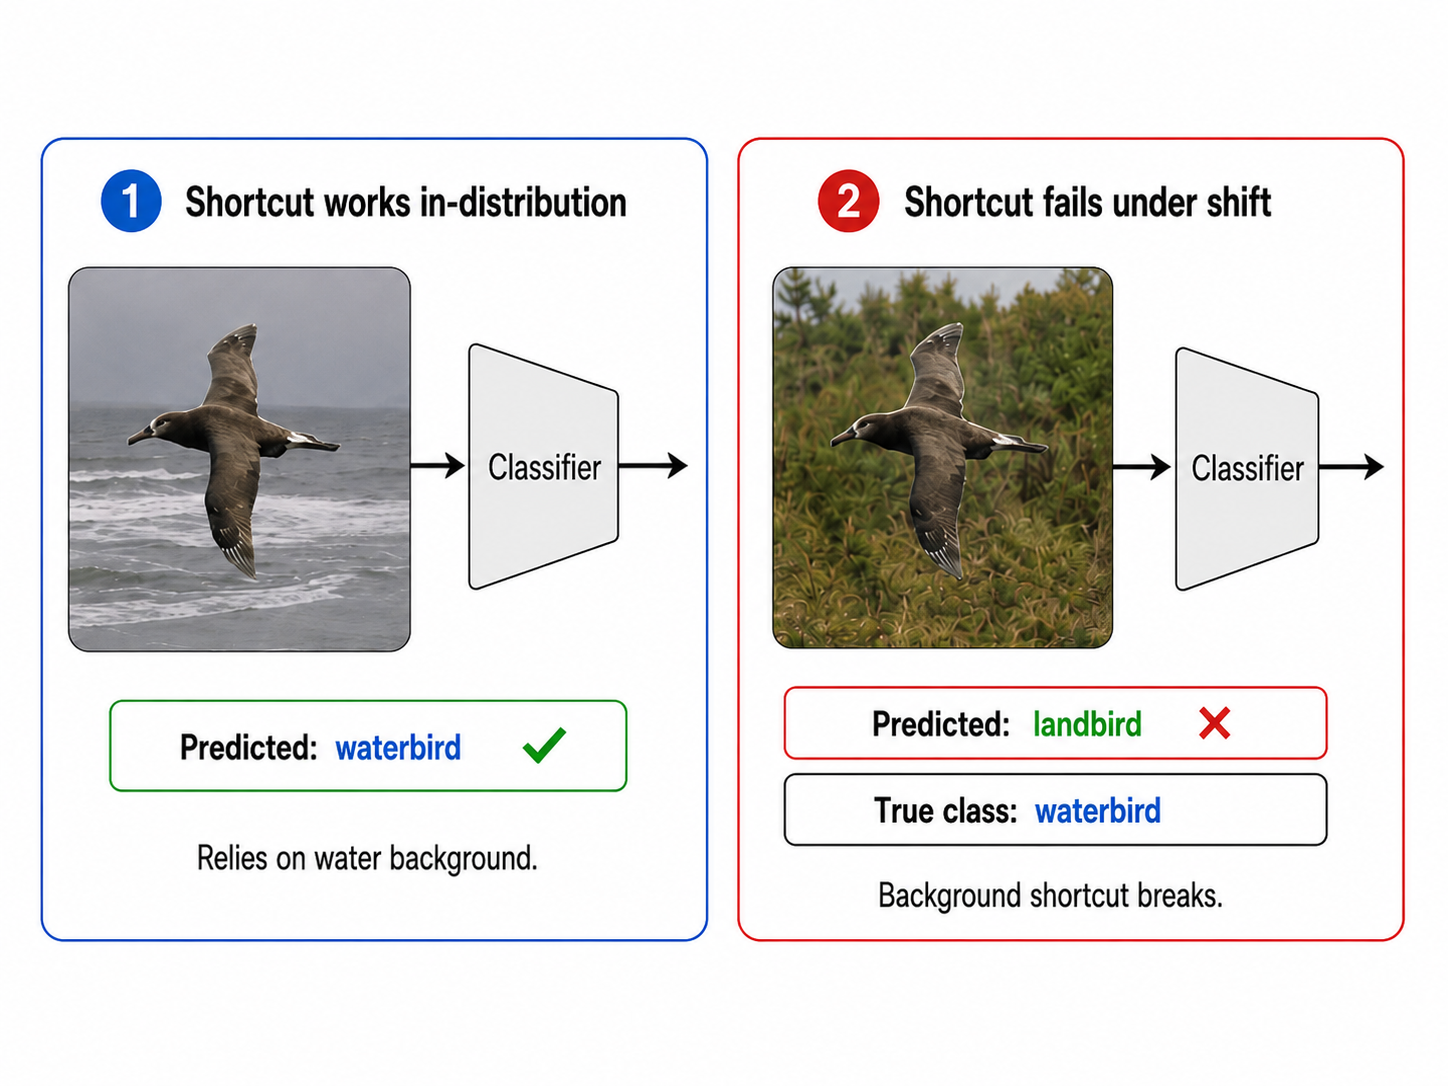
\includegraphics[width=0.95\linewidth]{figs/intro.png}
    \vspace{-3mm}
    \caption{\textbf{Shortcut learning under distribution shift.} When training data spuriously correlates class labels with background, a classifier may learn to use context rather than object evidence}
    \label{fig:intro}
\end{figure}

Vision--language models (VLMs)~\cite{lin2023clip} offer a scalable alternative source of spatial supervision. Because VLMs connect visual regions with natural-language concepts, they can provide weak localization cues from task-level prompts without requiring per-image human masks~\cite{elhoseiny2013write, frome2013devise, lampert2013attribute, le2020using, radford2021learning}. Recent work like GALS~\cite{petryk2022guiding} uses language-grounded spatial maps to guide classifier training, through input-gradient regularization. However, in shortcut-learning settings, gradient suppression is primarily a negative constraint: \textit{it tells the model where not to rely}. It does not directly specify where class evidence should be allocated. Moreover, input-gradient explanations can be noisy, and optimizing classification and explanation constraints jointly from the beginning can be unstable when shortcut features are highly predictive early in training.

In this work, we propose \textbf{Right for the Right Regions (R4RR)}, a training framework that converts VLM-derived localization into a positive, latent evidence-alignment signal for robust classification. Instead of penalizing input gradients on distracting pixels, R4RR aligns the student's spatial class evidence with a soft semantic localization map produced by a frozen VLM teacher~\cite{zhang2025frozen}. Concretely, the teacher provides a nonnegative task-relevant localization map from language prompts, while the student produces a spatial evidence map for the ground-truth class. We normalize both maps into spatial probability distributions and minimize a teacher-to-student KL divergence. This encourages the model to allocate class evidence to semantically relevant regions while preserving uncertainty in the teacher map, avoiding brittle hard masks.

A key component of R4RR is its \emph{Classify-then-Align} training schedule. We first train a model with cross-entropy to learn discriminative structure, then introduce evidence alignment and optimize the combined objective. Our curriculum ablations show that this schedule is substantially more effective than joint training from scratch or alignment-first training, especially in fully biased settings. We instantiate R4RR with CAM-style evidence maps from the final convolutional features for CNNs ~\cite{zhou2016learning}. Additionally, we show our framework also applies for Vision Transformers, where we construct a patch-space evidence map from transformer attention and patch-token activations, then apply the same distributional KL alignment objective.

%Early in training, CAMs or patch-level evidence maps can be noisy and poorly class-discriminative, making direct alignment unstable. R4RR therefore first learns a basic classifier using cross-entropy, then introduces the VLM-guided evidence alignment objective to redirect class evidence toward task-relevant regions. Our curriculum ablations show that this schedule is substantially more effective than joint training from scratch or alignment-first training, especially in fully biased settings.



We evaluate R4RR on three complementary benchmarks of shortcut learning and distribution shift: \emph{DecoyMNIST}~\cite{erion2021improving}, \emph{Waterbirds} \cite{sagawa2019distributionally}, and \emph{RedMeat}, derived from Food-101~\cite{bossard2014food}. Across all three datasets, \textbf{R4RR} consistently outperforms language-guided attention baseline, \emph{GALS}~\cite{petryk2022guiding}, attention-module baseline, \emph{ABN}~\cite{fukui2019attention}, robust-training baseline, \emph{AFR}~\cite{qiu2023simple}, representation-regularization baseline, \emph{ElRep}~\cite{wen2025elastic}, and standard empirical risk minimization (ERM) baselines. The gains are especially pronounced when training data provides little or no counter-bias evidence, as in the fully biased Waterbirds setting. We further show through Pointing Game~\cite{zhang2018top} that R4RR shifts model evidence toward task-relevant object regions.

Our contributions are:
\begin{enumerate}
\item We introduce \textbf{R4RR}, a VLM-guided training framework that improves shortcut robustness by aligning student spatial evidence with soft semantic localization maps from a frozen vision--language teacher.
\item We propose a positive latent evidence-alignment objective based on teacher-to-student KL divergence over spatial distributions, avoiding the limitations of hard masks and input-gradient suppression.
\item We introduce a practical \emph{Classify-then-Align} schedule and show that it substantially improves robustness over joint or alignment-first training.
\item We demonstrate that R4RR is architecture-general: it applies to ResNet, MobileNet, LeNet, and ViT students through architecture-specific spatial evidence maps.
\item We provide empirical evidence on DecoyMNIST, Waterbirds, and RedMeat showing improved worst-group robustness and better localization of task-relevant evidence.
\end{enumerate}

\section{Related Work}
\label{sec:related}

Right for the Right Reasons (RRR)~\cite{ross2017right} penalizes input gradients on features annotated as irrelevant, while CDEP~\cite{rieger2020interpretations} extends this idea using contextual-decomposition-based feature and interaction attributions. Other explanation-guided approaches use saliency, attention, or concept-level supervision to steer models toward interpretable evidence, including concept-sensitive objectives and human-in-the-loop correction mechanisms~\cite{gupta2023concept,gao2022aligning,schramowski2020making}. These methods require pixel-level masks, bounding boxes, curated concepts, or expert rationales creating a supervision bottleneck.

Earlier vision-and-language and zero-shot recognition methods condition classifiers on attributes or textual descriptions~\cite{elhoseiny2013write,frome2013devise,lampert2013attribute,radford2021learning}, while recent CLIP-based localization and weakly supervised segmentation methods show that language prompts can produce meaningful spatial cues~\cite{lin2023clip,zhang2024frozen}. The most closely related line of work uses these spatial cues to guide classifier attention. GALS~\cite{petryk2022guiding} grounds language specifications with a pretrained VLM and applies an auxiliary explanation regularization loss similar to  Right for the Right Reasons (RRR)~\cite{ross2017right}, discouraging reliance on distracting regions. PARIC~\cite{nautiyal2025paric} is a recent preprint that extends this direction by introducing probabilistic VLM embeddings. %: it samples from probabilistic image/text embeddings, generates multiple CLIP Grad-CAM maps, and aggregates them into a reference attention map for language-guided classification. PARIC focuses on uncertainty-aware attention-map generation and prediction stability, whereas our work focuses on how the spatial prior is used during student training for shortcut robustness.


Attention Branch Network (ABN)~\cite{fukui2019attention} augments a CNN with an attention branch whose output is used both for visualization and classification. Automatic Feature Reweighting (AFR)~\cite{qiu2023simple} improves group robustness by retraining the final layer of an ERM model with weights derived from the model's own errors, without requiring group labels. Elastic Representation (ElRep)~\cite{wen2025elastic} instead regularizes the learned representation to mitigate spurious correlations and improve group robustness. These approaches are complementary to R4RR.


% \paragraph{Architecture-specific and architecture-agnostic spatial evidence.}
% Most explanation-guided objectives are tied to a particular form of explanation, such as input gradients, saliency maps, or CNN attention maps. R4RR is instead formulated around a generic student spatial evidence map. For CNNs such as ResNet and MobileNet, this evidence can be instantiated using CAM-style maps from the final convolutional features~\cite{zhou2016learning}. For Vision Transformers, the same objective can be applied to patch-space evidence maps derived from transformer attention and patch-token activations. This makes R4RR an architecture-agnostic evidence-alignment framework: the teacher map, normalization, KL objective, and Classify-then-Align schedule remain unchanged, while only the student evidence-map construction depends on the architecture.

% \paragraph{From negative suppression to positive evidence allocation.}
% R4RR differs from prior language-guided attention regularization in its training mechanism. GALS and related RRR-style objectives primarily impose a negative constraint: they suppress gradients or attention on regions specified as distracting. In contrast, R4RR treats the VLM map as a soft spatial distribution over task-relevant regions and aligns the student's latent class evidence to this distribution using a teacher-to-student KL divergence. This provides a positive evidence-allocation signal, encouraging the model to place class evidence on semantic foreground regions rather than only penalizing evidence in the background. Our component ablations further separate map quality from training mechanism: replacing GALS maps with stronger VLM maps alone is insufficient, while applying the R4RR objective and schedule to alternative map sources recovers much of the robustness gain.

\section{Methodology}
\label{sec:method}

\subsection{Problem Setup}
Let $\mathcal{D}={(x_i,y_i)}_{i=1}^{N}$ denote a labeled image dataset, where $x_i\in\mathbb{R}^{H\times W\times 3}$ and $y_i\in{1,\ldots,C}$. We consider classification settings where task-irrelevant image regions, such as background, texture, border artifacts, or co-occurring context, are spuriously correlated with the label. A classifier trained only with empirical risk minimization may therefore achieve high training or average test accuracy while relying on these shortcut regions.

We train a student classifier $f_\theta$ that outputs logits $z_\theta(x)\in\mathbb{R}^{C}$ and predicted probabilities $p_\theta(x)=\mathrm{softmax}(z_\theta(x))$. Our goal is to learn a classifier that remains accurate while allocating its spatial evidence to task-relevant regions. We assume access to task-level language descriptions, but not to per-image human masks.

\subsection{Overview}
\label{sec:overview}

Our framework, \textbf{Right for the Right Regions (R4RR)}, uses a frozen vision--language teacher to provide soft spatial localization targets during training. For each training image $x_i$ and label $y_i$, R4RR constructs two maps:
\begin{itemize}
\item a \textbf{teacher localization map} $A^{\mathrm{VLM}}(x_i,y_i)$, produced by a frozen VLM-based localization pipeline from task-level language prompts;
\item a \textbf{student evidence map} $A^{\mathrm{stu}}_\theta(x_i,y_i)$, extracted from the student classifier and indicating where the student places evidence for class $y_i$.
\end{itemize}

R4RR aligns these maps by converting both to spatial probability distributions and minimizing a teacher-to-student KL divergence. This converts the VLM localization prior into a positive evidence-allocation signal: instead of only suppressing evidence in distracting regions (common in RRR-style regularization~\cite{ross2017right}), the student is encouraged to place class evidence on task-relevant regions.

The framework is architecture-agnostic. The teacher map, normalization, KL objective, and training schedule remain unchanged across students. Only the construction of $A^{\mathrm{stu}}_\theta$ depends on the student architecture. For CNNs such as ResNet~\cite{he2016deep} and MobileNetV2~\cite{sandler2018mobilenetv2}, we use CAM-style evidence maps. For ViT-B/16 students~\cite{dosovitskiy2020image}, we use an LGM-ViT-style~\cite{ben2024localization} patch-space evidence map.

\subsection{Teacher: Soft Semantic Localization Maps}
\label{sec:teacher}

For each dataset, we define a set of foreground terms $\mathcal{C}$ corresponding to task-relevant concepts and a set of background or context terms $\mathcal{B}$ corresponding to common distracting regions. These terms are inserted into natural-language prompt templates and encoded by a frozen vision--language model. Prompt details are provided in the supplementary pdf.

Our default teacher follows the WeCLIP+~\cite{zhang2024frozen} pipeline, using OpenAI CLIP with DINO refinement. Given an image $x$ and task-level foreground/background prompts, the teacher first obtains class-conditioned localization seeds using Grad-CAM~\cite{selvaraju2017grad} on the frozen CLIP visual backbone with respect to the text prototypes. These seeds are then refined using WeCLIP+'s refinement module (RFM+), which fuses CLIP and DINO~\cite{caron2021emerging} patch features and leverages CLIP attention to propagate and complete the CAM, producing a nonnegative soft localization map:
\begin{equation}
A^{\mathrm{VLM}}(x,y)\in\mathbb{R}^{H_{\mathrm{img}}\times W_{\mathrm{img}}}_{\ge 0}
\end{equation}

The teacher is used only during training. We precompute and cache teacher maps for the training split and freeze the teacher before student training. At inference time, only the student classifier is used. For our final evaluations, we additionally regenerate maps across seeded runs as a stricter robustness check, verifying that the gains are not tied to a single teacher-map instantiation. The total cached map storage is modest across all datasets; details are reported in the supplementary pdf.


\paragraph{Teacher map preprocessing.}
The teacher map is resized to the spatial resolution of the student evidence map using nearest-neighbor interpolation. Let the student evidence grid have resolution $H_s\times W_s$:
\begin{equation}
A^{\mathrm{VLM}}_{\downarrow}(x,y)
=
\mathrm{Downsample}_{\mathrm{NN}}\big(A^{\mathrm{VLM}}(x,y)\big)
\in
\mathbb{R}^{H_{\mathrm{s}}\times W_{\mathrm{s}}}_{\ge 0}.
\end{equation}

We then normalize the resized map into a spatial probability distribution:
\begin{equation}
\hat{A}^{\mathrm{VLM}}(x,y)[u,v]
=
\frac{A^{\mathrm{VLM}}_{\downarrow}(x,y)[u,v]}{\sum_{u',v'} A^{\mathrm{VLM}}_{\downarrow}(x,y)[u',v']+\epsilon}.
\end{equation}
This soft normalization avoids converting teacher maps into brittle hard masks and preserves uncertainty in the VLM localization prior.

\subsection{Student Spatial Evidence Maps}
\label{sec:student_maps}
R4RR requires a spatial evidence map from the student classifier for the ground-truth class, and the construction of this map depends on the student architecture. For CAM-compatible CNNs, we compute student evidence maps using Class Activation Mapping (CAM)~\cite{zhou2016learning} at the spatial resolution of the final convolutional block. We use standard CAM for ResNet-50~\cite{he2016deep} and MobileNetV2~\cite{sandler2018mobilenetv2}, both of which expose final convolutional features followed by global pooling and a linear classifier. For DecoyMNIST~\cite{erion2021improving}, we use Grad-CAM~\cite{selvaraju2017grad} on the second convolutional layer to match the LeNet-style architecture and prior protocol~\cite{rieger2020interpretations}. We discuss Vision Transformer-specific student evidence in Section~\ref{sec:ViTstudent}.


Let $F_\theta(x)\in\mathbb{R}^{D\times H_{\mathrm{s}}\times W_{\mathrm{s}}}$ denote the last convolutional feature tensor and let $\mathbf{W}\in\mathbb{R}^{C\times D}$ be the linear classifier weights (for $C$ classes). For an image $x$ and class $c$, the (pre-nonlinearity) CAM is
\begin{equation}
\begin{aligned}
\tilde{A}^{\mathrm{cam}}_\theta(x,c)[u,v]
&=
\sum_{d=1}^{D} \mathbf{W}_{c,d}\,F_\theta(x)[d,u,v],\\
&\quad (u,v)\in\{1,\dots,H_{\mathrm{s}}\}\times\{1,\dots,W_{\mathrm{s}}\}.
\end{aligned}
\end{equation}

We use the ground-truth class $c=y$ during training. To obtain a nonnegative spatial map, we apply ReLU followed by per-image min--max normalization.
% \begin{equation}
% A^{\mathrm{stu}}*\theta(x,y)[u,v]=
% \frac{
% R_\theta(x,y)[u,v]-\min_{u',v'}R_\theta(x,y)[u',v']
% }{
% \max_{u',v'}R_\theta(x,y)[u',v']-\min_{u',v'}R_\theta(x,y)[u',v']+\epsilon
% }.
% \end{equation}

After obtaining the student evidence map, we convert it into a spatial probability distribution. We first flatten the $H_s\times W_s$ map and apply a spatial softmax:
\begin{align}
\log \hat{A}^{\mathrm{stu}}_\theta(x,c)[u,v]
=
A^{\mathrm{stu}}_\theta(x,c)[u,v]
- \\ 
\log\!\sum_{u',v'} \exp\!\big(A^{\mathrm{stu}}_\theta(x,c)[u',v']\big).
\end{align}

\subsection{Training Objective}
\label{sec:objective}

The classification loss is standard cross-entropy:
\begin{equation}
\mathcal{L}_{\mathrm{CE}}(\theta)=-\frac{1}{B}
\sum_{i=1}^{B}
\log p_\theta(y_i\mid x_i).
\end{equation}

We align the student distribution to the teacher distribution using KL divergence in the teacher-to-student direction:
\begin{equation}
\mathcal{L}_{\mathrm{align}}(\theta)=\frac{1}{B}
\sum_{i=1}^{B}
\mathrm{KL}\left(
\hat{A}^{\mathrm{VLM}}(x_i,y_i)
\Vert
\hat{A}^{\mathrm{stu}}_\theta(x_i,y_i)
\right),
\end{equation}
where
\begin{equation}
\mathrm{KL}(P\Vert Q)=\sum_{u,v}P[u,v]\log\frac{P[u,v]}{Q[u,v]+\epsilon}.
\end{equation}

Unlike hard masking, the alignment loss does not force binary foreground/background decisions, and unlike input-gradient suppression, it directly specifies where class evidence should be allocated.


The final R4RR objective is
\begin{equation}
\mathcal{L}(\theta)=\mathcal{L}_{\mathrm{CE}}(\theta)
+
\lambda \mathcal{L}_{\mathrm{align}}(\theta),
\label{eq:r4rr_objective}
\end{equation}
where $\lambda>0$ controls the strength of evidence alignment.

\subsection{Classify-then-Align Curriculum}
\label{sec:classify_then_align}

Optimizing Eq.~\eqref{eq:r4rr_objective} from the beginning can be unstable because early student evidence maps are often noisy and poorly class-discriminative. R4RR therefore uses a two-phase \emph{Classify-then-Align} schedule.

\paragraph{Phase 1: classification warmup.}
We first train the student using only cross-entropy until the \emph{attention epoch} $E_{\mathrm{cls}}$:
\begin{equation}
\min_{\theta}\mathcal{L}_{\mathrm{CE}}(\theta).
\end{equation}

We treat $E_{\mathrm{cls}}$ (the epoch at which we activate evidence alignment) as a tunable hyperparameter selected on the validation set. This phase is not intended to eliminate shortcut reliance by itself. Its purpose is to produce minimally meaningful class evidence maps that can later be aligned with the VLM teacher.

\paragraph{Phase 2: evidence alignment.}
After the epoch $E_{\mathrm{cls}}$, we introduce the alignment objective and optimize
\begin{equation}
\min_{\theta}
\mathcal{L}_{\mathrm{CE}}(\theta)
+
\lambda \mathcal{L}_{\mathrm{align}}(\theta).
\end{equation}
This phase redirects the student's class evidence toward the teacher-localized task-relevant regions.

\textbf{Model selection.} We select checkpoints using validation performance after the alignment phase begins. This ensures that the selected model reflects the effect of evidence alignment rather than only the cross-entropy warmup. %Algorithm \ref{alg:r4rr} shows our approach. 


% \begin{algorithm}[t]
% \caption{R4RR Training with VLM-guided Evidence Alignment (Classify-then-Align)}
% \label{alg:r4rr}
% \begin{algorithmic}[1]
% \REQUIRE Dataset $\mathcal{D}$, teacher $\mathrm{VLM}$, prompts $\{\mathcal{T}_c\}_{c=1}^C$, alignment weight $\lambda$, attention epochs $E_{\mathrm{cls}}$, joint epochs $E_{\mathrm{joint}}$
% \STATE \textbf{Precompute teacher maps:} for each $(x_i,y_i)\in\mathcal{D}$ compute $A^{\mathrm{VLM}}(x_i,y_i)$ using $\mathrm{VLM}$ and prompts; store maps.
% \STATE Initialize CNN $f_\theta$.
% \STATE \textbf{Phase 1 (classification):} optimize $\mathcal{L}_{\mathrm{CE}}$ for $E_{\mathrm{cls}}$ epochs.
% \STATE Reset optimizer and scheduler; set the Phase~2 learning rate to $\eta_{\mathrm{joint}} = m \cdot \eta_{\mathrm{base}}$, where the multiplier $m$ is tuned.
% \STATE \textbf{Phase 2 (joint):} optimize $\mathcal{L}_{\mathrm{CE}}+\lambda\mathcal{L}_{\mathrm{align}}$ for $E_{\mathrm{joint}}$ epochs:
% \FOR{epoch $=1$ to $E_{\mathrm{joint}}$}
%     \FOR{minibatch $\{(x_i,y_i)\}_{i=1}^B$}
%         \STATE Compute logits $z_\theta(x_i)$ and $\mathcal{L}_{\mathrm{CE}}$.
%         \STATE Compute CAMs $A^{\mathrm{stu}}_\theta(x_i,y_i)$ and normalize to $\hat{A}^{\mathrm{stu}}_\theta$.
%         \STATE Downsample teacher maps $A^{\mathrm{VLM}}(x_i,y_i)$ to resolution of CAM $H_{\mathrm{s}}\times W_{\mathrm{s}}$ and normalize to $\hat{A}^{\mathrm{VLM}}(x_i,y_i)$.
%         \STATE Compute $\mathcal{L}_{\mathrm{align}}$.
%         \STATE Update $\theta$ using $\mathcal{L}=\mathcal{L}_{\mathrm{CE}}+\lambda\mathcal{L}_{\mathrm{align}}$.
%     \ENDFOR
% \ENDFOR
% \STATE \textbf{Inference:} use $f_\theta$ only (no teacher required).
% \end{algorithmic}
% \end{algorithm}

\section{Experiments}
\label{sec:experiment}

%We evaluate R4RR along three axes. First, we test whether evidence alignment improves robustness to spurious correlations on standard biased classification benchmarks. Second, we evaluate whether the learned evidence maps are better localized on task-relevant regions. Third, we test whether R4RR generalizes by applying the same framework to lightweight CNN and Vision Transformer students.

\subsection{Setup}
\label{sec:setup}

\textbf{Datasets.}
We evaluate our framework on three complementary benchmarks of shortcut learning: \textbf{DecoyMNIST}~\cite{erion2021improving},
\textbf{Waterbirds}~\cite{sagawa2019distributionally} and 
\textbf{RedMeat}~\cite{petryk2022guiding}. For Waterbirds, we evaluate two settings: Waterbirds$_{95}$ where a small fraction of training samples counter the dominant background-label correlation, and Waterbirds$_{100}$ where the label and background are perfectly correlated during training, making this setting challenging. Full dataset details and group/class counts are provided in the supplementary pdf.

\begin{figure*}[h]
\centering
\begin{tikzpicture}
\begin{groupplot}[
    group style={
        group size=2 by 2,
        horizontal sep=1.4cm,
        vertical sep=1.9cm
    },
    width=0.48\textwidth,
    height=0.31\textwidth,
    ybar,
    bar width=3.2pt,
    ymin=0,
    ymax=100,
    ylabel={Accuracy (\%)},
    symbolic x coords={Vanilla,CLIP-Z,CLIP-LR,ElRep,Upweight,ABN,GALS,AFR,R4RR},
    xtick=data,
    xticklabel style={rotate=45, anchor=east, font=\scriptsize},
    yticklabel style={font=\scriptsize},
    label style={font=\scriptsize},
    title style={font=\small},
    legend style={
        font=\scriptsize,
        at={(0.5,1.20)},
        anchor=south,
        legend columns=2,
        /tikz/every even column/.append style={column sep=0.3cm}
    },
    enlarge x limits=0.08,
    grid=major,
    grid style={dotted}
]

% ---------------- DecoyMNIST ----------------
\nextgroupplot[
    title={DecoyMNIST},
    legend to name=mainresultslegend
]
\addplot + [
    bar width = 8.5pt,
] coordinates {
    (Vanilla,45.9)
    (CLIP-Z,55.2)
    (CLIP-LR,88.3)
    (ElRep, 49.9)
    (Upweight,49.2)
    (ABN,80.8)
    (GALS,73.2)
    (AFR,44.6)
    (R4RR,96.6)
};
\addplot + [
    bar width = 8.5pt,
] coordinates {
    (Vanilla,0.0)
    (CLIP-Z,0.0)
    (CLIP-LR,76.2)
    (ElRep, 0.1)
    (Upweight,0.0)
    (ABN,25.2)
    (GALS,26.9)
    (AFR,0.0)
    (R4RR,95.8)
};
\legend{Mean group, Worst group}

% ---------------- Waterbirds-95 ----------------
\nextgroupplot[
    title={Waterbirds$_{95}$}
]
\addplot + [
    bar width = 8.5pt,
]coordinates {
    (Vanilla,87.1)
    (CLIP-Z,73.7)
    (CLIP-LR,80.4)
    (ElRep, 88.7)
    (Upweight,86.7)
    (ABN,84.5)
    (GALS,89.1)
    (AFR,91.9)
    (R4RR,90.2)
};
\addplot + [
    bar width = 8.5pt,
]coordinates {
    (Vanilla,71.2)
    (CLIP-Z,44.1)
    (CLIP-LR,56.2)
    (ElRep, 75.4)
    (Upweight,70.8)
    (ABN,62.9)
    (GALS,76.0)
    (AFR,90.4)
    (R4RR,87.1)
};

% ---------------- Waterbirds-100 ----------------
\nextgroupplot[
    title={Waterbirds$_{100}$}
]
\addplot + [
    bar width = 8.5pt,
]coordinates {
    (Vanilla,70.2)
    (CLIP-Z,73.4)
    (CLIP-LR,63.7)
    (ElRep, 74.0)
    (Upweight,70.9)
    (ABN,69.1)
    (GALS,79.9)
    (AFR,69.6)
    (R4RR,89.1)
};
\addplot + [
    bar width = 8.5pt,
]coordinates {
    (Vanilla,40.3)
    (CLIP-Z,43.8)
    (CLIP-LR,24.6)
    (ElRep, 39.8)
    (Upweight,32.9)
    (ABN,34.6)
    (GALS,57.2)
    (AFR,38.4)
    (R4RR,84.8)
};

% ---------------- RedMeat ----------------
\nextgroupplot[
    title={RedMeat}
]
\addplot + [
    bar width = 8.5pt,
]coordinates {
    (Vanilla,67.3)
    (CLIP-Z,61.5)
    (CLIP-LR,76.6)
    (ElRep, 68.1)
    (Upweight,68.3)
    (ABN,65.6)
    (GALS,71.9)
    (AFR,60.7)
    (R4RR,73.2)
};
\addplot + [
    bar width = 8.5pt,
]coordinates {
    (Vanilla,48.0)
    (CLIP-Z,5.6)
    (CLIP-LR,54.0)
    (ElRep, 49.0)
    (Upweight,47.9)
    (ABN,55.3)
    (GALS,57.0)
    (AFR,58.2)
    (R4RR,60.9)
};

\end{groupplot}
\end{tikzpicture}

\vspace{-0.3em}
\ref{mainresultslegend}

\vspace{-0.5em}
\caption{
\textbf{Main robustness results across datasets.}
We compare standard ERM (\textbf{Vanilla}), class-balanced training (\textbf{Upweight}), zero-shot CLIP (\textbf{CLIP-Z}), linear probing on CLIP features (\textbf{CLIP-LR}), ElRep, ABN, GALS, AFR, and our method (\textbf{R4RR}).
Each panel reports mean group accuracy and worst-group accuracy, averaged over five seeds where applicable. Higher is better.
Exact values and standard deviations are provided in the supplementary material.
}
\label{fig:main_results}
\end{figure*}





\textbf{Baselines.} \textbf{Vanilla} trains the student using standard cross-entropy. \textbf{Upweight}~\cite{petryk2022guiding} uses class-balanced cross-entropy with weights inversely proportional to class frequency. \textbf{CLIP-${Zero}$} and \textbf{CLIP-${LR}$} use OpenAI CLIP RN50~\cite{radford2021learning}. CLIP-${Zero}$ evaluates the frozen model with zero-shot text prompts for the target classes, while CLIP-${LR}$ trains a linear classifier on frozen CLIP image features. Direct zero-shot results for all teacher VLM variants are provided in the supplementary material. \textbf{GALS}~\cite{petryk2022guiding} uses language-grounded maps to guide a classifier through explanation regularization. For GALS, we report the strongest validation-selected variant across tuned CLIP backbones and attention-supervision mechanisms. \textbf{ABN}~\cite{fukui2019attention} augments a CNN with an attention branch trained jointly with the classifier. \textbf{AFR}~\cite{qiu2023simple} starts from an ERM-trained model and retrains the final layer with an automatically weighted loss that emphasizes samples the ERM model predicts poorly. \textbf{ElRep}~\cite{wen2025elastic} adds nuclear- and Frobenius-norm penalties to the learned representation to reduce spurious feature reliance.




\textbf{Metrics.} Following group-robustness evaluation~\cite{sagawa2019distributionally}, we report two group-level metrics: (i) \emph{average group accuracy} (\textbf{Mean$_{Group}$}), which assigns equal weight to each group regardless of frequency, and (ii) \emph{worst-group accuracy}, defined as the minimum accuracy over the four groups (\textbf{Worst$_{Group}$}). Worst-group accuracy is particularly informative because it reflects performance on the minority and bias-conflicting groups (e.g. \emph{waterbird-on-land} in Waterbirds dataset), which degrade most severely when the model relies on spurious background cues. For Waterbirds, groups correspond to the four combinations of bird type and background. For DecoyMNIST, groups correspond to digit classes. For RedMeat, groups correspond to the five target classes. 

\textbf{Student details.} Our main experiments use the same student architectures as prior work for each benchmark. For Waterbirds and RedMeat, we train an ImageNet-pretrained ResNet-50~\cite{he2016deep}. For DecoyMNIST, we train a LeNet-style CNN~\cite{lecun1998gradient}. To test architecture generality, we additionally evaluate R4RR with MobileNetV2~\cite{sandler2018mobilenetv2} and ViT-B/16 students in Section \ref{sec:archgeneralize}. We provide exact training details in the supplementary pdf. 
%R4RR uses a two-phase training schedule. In the first phase, the student is trained with cross-entropy only. In the second phase, we optimize cross-entropy plus the VLM-guided evidence-alignment loss. The teacher maps are precomputed and cached before student training, and the teacher is not used during inference.



\textbf{Hyperparameters and evaluation.}
For each dataset and method, we select hyperparameters using automated validation-based tuning unless otherwise noted. 
For the main ResNet/LeNet experiments and baseline comparisons, we run 50 Optuna~\cite{akiba2019optuna} trials per \emph{(dataset, method)} configuration and choose the best trial by validation performance. 
For the architecture-transfer experiments with MobileNetV2 and ViT-B/16 students, we use a smaller 25-trial Optuna budget per configuration.
Unless otherwise noted, all classification results are reported as mean$\pm$standard deviation over five random seeds.
We provide full hyperparameter optimization details in the supplementary material and release the validation-selected hyperparameters for all methods, variants, and ablations in the accompanying code.

\subsection{Results}\label{sec:results}

Figure~\ref{fig:main_results} shows the comparison between different methods. Due to page constraints, we provide qualitative examples in the supplementary pdf. 

\textbf{DecoyMNIST.} Standard ERM (\textbf{Vanilla}) and class reweighting (\textbf{Upweight}) collapse completely on the bias-conflicting groups, indicating near-total reliance on the decoy cue. Zero-shot CLIP (\textbf{CLIP$-{Z}$}) shows the same failure mode on worst-group accuracy despite improved average performance. In contrast, our method \textbf{(R4RR)} achieves the highest per-group and worst-group accuracy, substantially outperforming all baselines we compare against. 

% \begin{table}[h]
% \caption{DecoyMNIST performance evaluation with test accuracy (mean$\pm$std over 5 runs) comparing standard ERM trained model (\textbf{Vanilla}), class-balanced (\textbf{Upweight}), zero-shot CLIP classifier (\textbf{\textbf{CLIP$_{Zero}$}}), linear probe on CLIP features (\textbf{\textbf{CLIP$_{LR}$}}), \textbf{GALS}~\cite{petryk2022guiding}, \textbf{ABN}~\cite{fukui2019attention}, \textbf{AFR}~\cite{qiu2023simple}, and our proposed method (\textbf{Ours}). Higher is better.}
% \label{tab:decoymnist}
% \resizebox{0.5\textwidth}{!}{%
% \begin{tabular}{@{}lcccccccc@{}}
% \toprule
%  &
%   \textbf{Vanilla} &
%  \textbf{CLIP$_{Zero}$} &
%  \textbf{CLIP$_{LR}$} &
%   \textbf{Upweight} &
%   \textbf{ABN} &
%   \textbf{GALS} &
%   \textbf{AFR} &
%   \textbf{Ours} \\ \midrule
% \textbf{Per$_{Group}$} &
%   45.9\scriptsize$\pm$2.7 &
%   55.2\scriptsize$\pm$0.0 &
%   88.3\scriptsize$\pm$0.0 &
%   49.2\scriptsize$\pm$3.2 &
%   80.8\scriptsize$\pm$6.0 &
%   73.2\scriptsize$\pm$11.3 &
%   44.6\scriptsize$\pm$3.2 &
%   \textbf{96.6\scriptsize$\pm$0.1} \\
% \textbf{Worst$_{Group}$} &
%   0.00\scriptsize$\pm$0.0 &
%   0.00\scriptsize$\pm$0.0 &
%   76.2\scriptsize$\pm$0.0 &
%   0.0\scriptsize$\pm$0.0 &
%   25.2\scriptsize$\pm$17.0 &
%   26.9\scriptsize$\pm$22.8 &
%   0.0\scriptsize$\pm$0.0 &
%   \textbf{95.8\scriptsize$\pm$1.3} \\ \bottomrule
% \end{tabular}%
% }
% \end{table}

\textbf{Waterbirds.}
On Waterbirds$_{95}$, where a small fraction of counter-bias examples is available, AFR performs strongly and R4RR remains competitive while substantially improving over ERM.
The gap is largest on Waterbirds$_{100}$, where background and label are perfectly correlated during training.
In this setting, ERM, class balancing, ABN, AFR, ElRep, and direct VLM classifiers all remain vulnerable to the background shortcut, while R4RR achieves the strongest mean-group and worst-group accuracy.
This suggests that when the training distribution provides no evidence that the shortcut is unreliable, the VLM-derived spatial prior supplies a useful corrective signal, redirecting the student toward bird evidence rather than background evidence.


\textbf{RedMeat.} R4RR improves worst-group accuracy over ERM, class balancing, GALS, ABN, AFR, ElRep, and direct VLM classifiers. CLIP$_{LR}$ obtains the highest mean group accuracy, indicating that frozen CLIP features are strong for average classification on this dataset. However, R4RR obtains the best worst-group accuracy, suggesting that explicitly training the classifier to allocate evidence to the target food region improves robustness on the most difficult classes. 


\subsection{Does R4RR improve localization?}\label{sec:pointing}

Beyond classification performance, we assess whether our training procedure improves \emph{where} the model attends, i.e., whether its explanations concentrate on task-relevant evidence. We use the \emph{Pointing Game} \cite{zhang2018top}, a standard protocol for evaluating spatial explanations. For each input image $x_i$, the Pointing Game requires (i) an explanation map $a_i \in \mathbb{R}^{H\times W}$ produced by the model, and (ii) a binary mask $Z_i \in \{0,1\}^{H\times W}$ indicating task-relevant pixels. A sample is counted as a \emph{hit} if the location of the maximum explanation value lies inside the mask. The Pointing Game score is the average hit rate over the evaluation set. Intuitively, a higher score indicates that the model's peak evidence aligns with the relevant region, suggesting that the model is ``right for the right regions'' rather than relying on spurious context. We use the bird segmentation masks in Waterbirds-95\% and Waterbirds-100\% to define $Z_i$. We report Pointing Game on the validation-selected seed for each method. Figure~\ref{fig:pointing_game} shows that R4RR achieves the highest Pointing Game score in both Waterbirds settings. 


\begin{figure}[t]
\centering
\begin{tikzpicture}
\begin{groupplot}[
    group style={
        group size=2 by 1,
        horizontal sep=1.2cm
    },
    width=0.55\columnwidth,
    height=0.54\columnwidth,
    ybar,
    bar width=5pt,
    ymin=0,
    ymax=100,
    ylabel={Hit rate (\%)},
    symbolic x coords={Vanilla,CLIP-Z,CLIP-LR,ElRep,Upweight,ABN,GALS,AFR,R4RR},
    xtick=data,
    xticklabel style={rotate=60, anchor=east, font=\scriptsize},
    yticklabel style={font=\scriptsize},
    label style={font=\scriptsize},
    title style={font=\small},
    enlarge x limits=0.08,
    grid=major,
    grid style={dotted}
]

% -------- Waterbirds-95 --------
\nextgroupplot[
    title={Waterbirds$_{95}$}
]
\addplot + [
    bar width = 7.5pt,
] coordinates {
    (Vanilla,59.9)
    (CLIP-Z,32.4)
    (CLIP-LR,53.5)
    (ElRep,66.0)
    (Upweight,67.4)
    (ABN,7.8)
    (GALS,69.4)
    (AFR,63.9)
    (R4RR,76.6)
};

% -------- Waterbirds-100 --------
\nextgroupplot[
    title={Waterbirds$_{100}$}
]
\addplot + [
    bar width = 7.5pt,
] coordinates {
    (Vanilla,46.5)
    (CLIP-Z,32.0)
    (CLIP-LR,36.4)
    (ElRep,61.1)
    (Upweight,59.3)
    (ABN,6.5)
    (GALS,59.3)
    (AFR,61.6)
    (R4RR,74.7)
};

\end{groupplot}
\end{tikzpicture}

\vspace{-0.5em}
\caption{
\textbf{Pointing Game evaluation on Waterbirds.}
Hit rate (\%) measures whether the peak activation of the explanation map falls inside the ground-truth bird segmentation mask. Higher is better.
%R4RR achieves the best localization performance on both Waterbirds$_{95}$ and Waterbirds$_{100}$, indicating that evidence alignment improves not only robustness but also spatial grounding on task-relevant object regions.
}
\label{fig:pointing_game}
\end{figure}



\subsection{Architecture Generalization}
\label{sec:archgeneralize}

%The main experiments use LeNet~\cite{lecun1998gradient} and ResNet-50~\cite{he2016deep}. We therefore evaluate R4RR on two additional student families: MobileNet~\cite{howard2017mobilenets}, representing lightweight CNNs, and ViT-B/16, representing transformer-based image classifiers.

\subsubsection{MobileNetV2}






We test architecture transfer by replacing the ResNet-50 student with an ImageNet-pretrained MobileNetV2~\cite{sandler2018mobilenetv2}. R4RR keeps the same teacher maps, KL alignment loss, Classify$\rightarrow$Align schedule, training length, and checkpoint-selection rule. We make MobileNetV2 CAM-compatible by using its final convolutional feature map with a dropout-free GAP+linear head, allowing the same class-specific CAM evidence construction used for ResNet-50. Figure~\ref{fig:mobilenet_transfer} shows that R4RR also improves MobileNetV2 robustness over vanilla training, with the largest gains appearing in worst-group accuracy.

\begin{figure}[t]
\centering
\begin{tikzpicture}
\begin{groupplot}[
    group style={
        group size=3 by 1,
        horizontal sep=0.08cm
    },
    scale only axis,
    width=0.30\columnwidth,
    height=0.32\columnwidth,
    ybar,
    bar width=5.5pt,
    ymin=25,
    ymax=95,
    symbolic x coords={ERM,R4RR},
    xtick=data,
    xticklabel style={font=\scriptsize},
    yticklabel style={font=\scriptsize},
    label style={font=\scriptsize},
    title style={font=\small},
    enlarge x limits=0.55,
    grid=major,
    grid style={dotted},
    error bars/y dir=both,
    error bars/y explicit,
    legend style={
        font=\scriptsize,
        at={(1.58,1.20)},
        anchor=south,
        legend columns=2
    }
]

\nextgroupplot[
    title={Waterbirds$_{95}$},
    ylabel={Accuracy (\%)},
    legend to name=mobilenettransferlegend
]
\addplot coordinates {
    (ERM,81.2) +- (0,0.4)
    (R4RR,86.6) +- (0,0.7)
};
\addplot coordinates {
    (ERM,55.3) +- (0,1.9)
    (R4RR,66.3) +- (0,1.8)
};
\legend{Mean group, Worst group}

\nextgroupplot[
    title={Waterbirds$_{100}$},
    yticklabels=\empty,
    ylabel={}
]
\addplot coordinates {
    (ERM,70.9) +- (0,1.3)
    (R4RR,80.4) +- (0,1.1)
};
\addplot coordinates {
    (ERM,35.0) +- (0,7.0)
    (R4RR,53.8) +- (0,4.3)
};

\nextgroupplot[
    title={RedMeat},
    yticklabels=\empty,
    ylabel={}
]
\addplot coordinates {
    (ERM,67.2) +- (0,0.5)
    (R4RR,71.4) +- (0,0.8)
};
\addplot coordinates {
    (ERM,47.0) +- (0,2.5)
    (R4RR,52.8) +- (0,3.3)
};

\end{groupplot}
\end{tikzpicture}

\vspace{0.10em}
\ref{mobilenettransferlegend}

\vspace{-0.55em}

\caption{
\textbf{MobileNetV2 architecture transfer.}
With a MobileNetV2 student, R4RR still improves over ERM while using CAM-based evidence maps.
}
\label{fig:mobilenet_transfer}
\end{figure}

\subsubsection{Vision Transformer}\label{sec:ViTstudent}

For ViT-B/16 students~\cite{dosovitskiy2020image}, CNN-style CAM is not directly available because the model operates on patch tokens rather than convolutional feature maps. We therefore use a ViT-native patch-space evidence map adapted from the embedding-attention fused explanation map of LGM-ViT~\cite{ben2024localization}. This changes only the student evidence extractor: the VLM teacher maps, teacher-to-student KL loss, and Classify$\rightarrow$Align schedule are unchanged.

Let the final transformer block contain $M$ attention heads and $P=H_sW_s$ patch tokens. We extract two patch-level signals. First, from the final-layer attention tensor $\mathcal{A}^{L}\in\mathbb{R}^{M\times(P+1)\times(P+1)}$, where token $0$ is the CLS token, we compute the averaged CLS-to-patch attention
\begin{equation}
a_p(x)=\frac{1}{M}\sum_{m=1}^{M}\mathcal{A}^{L}_{m,0,p}.
\end{equation}
Second, from the final patch tokens $h_p\in\mathbb{R}^{D}$, we compute an embedding-activation score
\begin{equation}
b_p(x)=\frac{1}{D}\sum_{d=1}^{D}h_{p,d}.
\end{equation}
The ViT evidence score is their weighted fusion,
\begin{equation}
s_p(x)=\beta a_p(x)+(1-\beta)b_p(x),
\end{equation}
with $\beta=0.85$ in our experiments. We reshape $\{s_p\}_{p=1}^{P}$ into an $H_s\times W_s$ patch grid and use it as $A^{\mathrm{stu}}_\theta(x)$ in the same spatial KL alignment objective as the CNN students.


Figure~\ref{fig:vit_transfer} shows that R4RR transfers beyond CNN students: replacing CAMs with a transformer-native patch evidence map still improves ViT robustness across all datasets. The gains are largest on Waterbirds$_{100}$, where no counter-bias examples are available during training, suggesting that the VLM-derived spatial prior remains useful even when evidence is represented over patch tokens rather than convolutional feature maps. These results support R4RR as an architecture-general evidence-alignment framework rather than a CAM-specific CNN regularizer.


\begin{figure}[t]
\centering
\begin{tikzpicture}
\begin{groupplot}[
    group style={
        group size=3 by 1,
        horizontal sep=0.08cm
    },
    scale only axis,
    width=0.30\columnwidth,
    height=0.32\columnwidth,
    ybar,
    bar width=5.5pt,
    ymin=25,
    ymax=95,
    symbolic x coords={ERM,R4RR},
    xtick=data,
    xticklabel style={font=\scriptsize},
    yticklabel style={font=\scriptsize},
    label style={font=\scriptsize},
    title style={font=\small},
    enlarge x limits=0.55,
    grid=major,
    grid style={dotted},
    error bars/y dir=both,
    error bars/y explicit,
    legend style={
        font=\scriptsize,
        at={(1.58,1.20)},
        anchor=south,
        legend columns=2
    }
]

\nextgroupplot[
    title={Waterbirds$_{95}$},
    ylabel={Accuracy (\%)},
    legend to name=vittransferlegend
]
\addplot coordinates {
    (ERM,79.4) +- (0,0.7)
    (R4RR,86.1) +- (0,1.2)
};
\addplot coordinates {
    (ERM,55.9) +- (0,3.0)
    (R4RR,72.1) +- (0,4.5)
};
\legend{Mean group, Worst group}

\nextgroupplot[
    title={Waterbirds$_{100}$},
    yticklabels=\empty,
    ylabel={}
]
\addplot coordinates {
    (ERM,69.6) +- (0,0.6)
    (R4RR,83.2) +- (0,0.5)
};
\addplot coordinates {
    (ERM,36.8) +- (0,2.4)
    (R4RR,61.8) +- (0,2.6)
};

\nextgroupplot[
    title={RedMeat},
    yticklabels=\empty,
    ylabel={}
]
\addplot coordinates {
    (ERM,68.1) +- (0,0.4)
    (R4RR,73.1) +- (0,0.5)
};
\addplot coordinates {
    (ERM,49.4) +- (0,3.2)
    (R4RR,56.8) +- (0,2.4)
};

\end{groupplot}
\end{tikzpicture}

\vspace{0.1em}
\ref{vittransferlegend}

\vspace{-0.55em}
\caption{
\textbf{R4RR transfers to ViT-B/16 students.}
Using an EAFEM-style patch-space evidence map, R4RR improves over ViT ERM.
}
\label{fig:vit_transfer}
\end{figure}




\section{Ablation studies}\label{sec:ablation}

\subsection{Study on teacher selection}
\begin{figure}[t]
\centering
\begin{tikzpicture}
\begin{groupplot}[
    group style={
        group size=1 by 2,
        vertical sep=1.85cm
    },
    width=0.93\columnwidth,
    height=0.43\columnwidth,
    ybar,
    bar width=5pt,
    ymin=75,
    ymax=93,
    ylabel={Accuracy (\%)},
    symbolic x coords={CLIP+DINO,OCLIP+DINO,SigLIP2+DINO,CLIP+XCiT},
    xtick=data,
    xticklabel style={rotate=25, anchor=east, font=\scriptsize},
    yticklabel style={font=\scriptsize},
    label style={font=\scriptsize},
    title style={font=\small},
    legend style={
        font=\scriptsize,
        at={(0.5,1.22)},
        anchor=south,
        legend columns=2
    },
    enlarge x limits=0.13,
    grid=major,
    grid style={dotted},
    error bars/y dir=both,
    error bars/y explicit
]
% ---------------- Waterbirds-95 ----------------
\nextgroupplot[
    title={Waterbirds$_{95}$},
    legend to name=teacherlegend
]
\addplot+[error bars/.cd, y dir=both, y explicit] coordinates {
    (CLIP+DINO,90.2) +- (0,0.7)
    (OCLIP+DINO,90.5) +- (0,0.3)
    (SigLIP2+DINO,90.3) +- (0,0.3)
    (CLIP+XCiT,90.4) +- (0,0.3)
};
\addplot+[error bars/.cd, y dir=both, y explicit] coordinates {
    (CLIP+DINO,87.1) +- (0,2.7)
    (OCLIP+DINO,88.1) +- (0,0.9)
    (SigLIP2+DINO,87.4) +- (0,0.9)
    (CLIP+XCiT,88.0) +- (0,1.2)
};
\legend{Mean group, Worst group}

% ---------------- Waterbirds-100 ----------------
\nextgroupplot[
    title={Waterbirds$_{100}$}
]
\addplot+[error bars/.cd, y dir=both, y explicit] coordinates {
    (CLIP+DINO,89.1) +- (0,0.4)
    (OCLIP+DINO,89.1) +- (0,0.5)
    (SigLIP2+DINO,88.0) +- (0,0.8)
    (CLIP+XCiT,89.1) +- (0,0.3)
};
\addplot+[error bars/.cd, y dir=both, y explicit] coordinates {
    (CLIP+DINO,84.8) +- (0,1.0)
    (OCLIP+DINO,85.6) +- (0,1.8)
    (SigLIP2+DINO,81.6) +- (0,0.8)
    (CLIP+XCiT,84.0) +- (0,1.3)
};

\end{groupplot}
\end{tikzpicture}
\vspace{-0.4em}
\ref{teacherlegend}
\vspace{-0.15em}
\caption{
\textbf{Teacher ablation on Waterbirds.}
We vary the VLM backbone and refinement backbone while keeping the student, loss, and training curriculum fixed.
\textbf{OCLIP+DINO} denotes OpenCLIP with DINO refinement, and \textbf{CLIP+XCiT} denotes CLIP with XCiT-DINO refinement.
%R4RR is relatively stable across teacher choices; OpenCLIP+DINO is slightly strongest on worst-group accuracy, while SigLIP2+DINO drops more in the fully biased Waterbirds$_{100}$ setting.
}
\label{fig:teacher_ablation}
\end{figure}



Our default teacher follows WeCLIP+~\cite{zhang2024frozen}, which combines CLIP and DINO. Here, we test the sensitivity of \textbf{R4RR} to the teacher by swapping (i) the VLM backbone (CLIP $\rightarrow$ OpenCLIP~\cite{openclip} with LAION-pretrained weights or SigLIP2~\cite{siglip2}) and (ii) the refinement backbone (DINO $\rightarrow$ XCiT-DINO~\cite{el2021xcit, caron2021emerging}), while keeping the student, prompts, loss, and curriculum fixed.

Figure~\ref{fig:teacher_ablation} shows that \textbf{R4RR} is largely insensitive to the teacher choice: all variants maintain strong Mean$_{Group}$ accuracy in both bias settings. OpenCLIP is consistently best (or tied) on Worst$_{Group}$, while SigLIP2 drops on Waterbirds$_{100}$, suggesting that teacher calibration matters most when training is fully biased. This trend carries over to other datasets, discussed in the supplementary pdf.

\subsection{Sensitivity to hyperparameters and teacher-map quality}
\label{sec:sensitivity_stress}


We further test whether \textbf{R4RR} depends on a fragile operating point or perfectly accurate teacher maps. First, we perform a local sensitivity study on Waterbirds$_{100}$ by perturbing one \textbf{R4RR}-specific hyperparameter at a time around the validation-selected configuration: the alignment start epoch, the KL alignment weight, and the Phase-2 learning-rate multiplier. 
Across these perturbations, performance remains stable: mean group accuracy stays within $88.4$--$89.1$, and worst-group accuracy stays within $82.5$--$85.1$, compared to $89.1\pm0.4$ mean group and $84.8\pm1.0$ worst-group accuracy for the tuned configuration. Full sensitivity details are provided in the supplementary pdf. 

Second, we stress-test \textbf{R4RR} under imperfect teacher supervision by corrupting a fixed 15\% subset of training teacher maps before student training. We consider two corruption types: aggressive Gaussian blur, which makes the teacher map spatially diffuse, and inversion, which creates an actively misleading teacher signal. \textbf{R4RR} remains stable across all datasets, with the largest worst-group drop occurring on RedMeat, the noisiest benchmark, while Waterbirds and DecoyMNIST show little to no degradation. These results indicate that \textbf{R4RR} benefits from the overall structure of teacher-guided evidence alignment rather than relying on a razor-thin hyperparameter setting or perfectly accurate teacher maps for every training example. Full corruption details are provided in the supplementary pdf.

\subsection{Teacher maps vs.\ objective/schedule}
\label{sec:ablation_gals_vs_r4rr}
To disentangle why \textbf{R4RR} improves over GALS~\cite{petryk2022guiding} which also uses VLM-guided maps, we factor the gain into (i) the \emph{training mechanism} (our KL evidence-alignment with a two-phase warm-start) and (ii) the \emph{teacher map construction} (WeCLIP+~\cite{zhang2024frozen}). We compare: (A) \emph{GALS objective + our teacher maps}, (B) \emph{R4RR objective/schedule + GALS RN50 maps}, (C) \emph{R4RR objective/schedule + GALS maps}, (D) \emph{R4RR (ours)}: R4RR objective/schedule + teacher maps.

\begin{figure}[t]
\centering
\begin{tikzpicture}
\begin{groupplot}[
    group style={
        group size=1 by 3,
        vertical sep=1.1cm
    },
    width=0.93\columnwidth,
    height=0.34\columnwidth,
    ybar,
    bar width=6pt,
    ymin=40,
    ymax=95,
    ylabel={Accuracy (\%)},
    symbolic x coords={A,B,C,D},
    xtick=data,
    xticklabels={A,B,C,D},
    xticklabel style={font=\scriptsize},
    yticklabel style={font=\scriptsize},
    label style={font=\scriptsize},
    title style={font=\small},
    legend style={
        font=\scriptsize,
        at={(0.5,1.22)},
        anchor=south,
        legend columns=2
    },
    enlarge x limits=0.18,
    grid=major,
    grid style={dotted},
    error bars/y dir=both,
    error bars/y explicit
]

% ---------------- Waterbirds-95 ----------------
\nextgroupplot[
    title={Waterbirds$_{95}$},
    legend to name=galsr4rrlegend
]
\addplot+[error bars/.cd, y dir=both, y explicit] coordinates {
    (A,87.0) +- (0,0.4)
    (B,89.4) +- (0,0.3)
    (C,86.1) +- (0,1.5)
    (D,90.2) +- (0,0.7)
};
\addplot+[error bars/.cd, y dir=both, y explicit] coordinates {
    (A,70.4) +- (0,2.6)
    (B,83.8) +- (0,1.5)
    (C,71.6) +- (0,4.7)
    (D,87.1) +- (0,2.7)
};
\legend{Mean group, Worst group}

% ---------------- Waterbirds-100 ----------------
\nextgroupplot[
    title={Waterbirds$_{100}$}
]
\addplot+[error bars/.cd, y dir=both, y explicit] coordinates {
    (A,73.2) +- (0,2.2)
    (B,87.7) +- (0,0.3)
    (C,85.4) +- (0,0.1)
    (D,89.1) +- (0,0.5)
};
\addplot+[error bars/.cd, y dir=both, y explicit] coordinates {
    (A,40.9) +- (0,9.4)
    (B,76.2) +- (0,1.7)
    (C,72.6) +- (0,2.0)
    (D,85.6) +- (0,1.8)
};

% ---------------- RedMeat ----------------
\nextgroupplot[
    title={RedMeat}
]
\addplot+[error bars/.cd, y dir=both, y explicit] coordinates {
    (A,71.8) +- (0,0.7)
    (B,68.9) +- (0,1.5)
    (C,67.4) +- (0,1.1)
    (D,73.2) +- (0,1.0)
};
\addplot+[error bars/.cd, y dir=both, y explicit] coordinates {
    (A,57.4) +- (0,2.2)
    (B,52.3) +- (0,6.2)
    (C,51.0) +- (0,2.4)
    (D,60.9) +- (0,3.4)
};

\end{groupplot}
\end{tikzpicture}

\vspace{0.1em}
\ref{galsr4rrlegend}

\vspace{-0.5em}
\caption{
\textbf{GALS vs.\ R4RR component ablation.}
We separate the effects of the teacher-map source and the training objective/schedule.
\textbf{(A)} GALS objective + our teacher maps.
\textbf{(B)} R4RR objective/schedule + GALS RN50 maps.
\textbf{(C)} R4RR objective/schedule + GALS ViT maps.
\textbf{(D)} Full R4RR: R4RR objective/schedule + our teacher maps.
%Across datasets, replacing the training mechanism yields a larger gain than replacing the teacher maps alone, and the full combination performs best overall.
}
\label{fig:gals_r4rr_ablation}
\end{figure}


Figure~\ref{fig:gals_r4rr_ablation} shows that map quality alone is not sufficient: \textbf{GALS + our maps (A)} remains brittle under full bias (Waterbirds$_{100}$ worst-group $40.9$). In contrast, swapping \emph{only} the training mechanism (\textbf{R4RR objective + GALS maps (B--C)}) recovers most of the robustness on Waterbirds, indicating that aligning {latent} evidence under a warm-started two-phase schedule is the primary driver. Finally, \textbf{R4RR} with WeCLIP+ maps performs best across datasets, suggesting the two components are complementary: our schedule provides the main robustness gain, while segmentation-style pseudo-masks further strengthen the alignment target, especially in the fully biased and noisy settings.


\subsection{Training curriculum}
\label{sec:ablationtrainingcuriculum}

R4RR uses a two-phase \textbf{Classify$\rightarrow$Align} schedule: the student first learns with $\mathcal{L}_{\mathrm{CE}}$, then optimizes $\mathcal{L}_{\mathrm{CE}}+\lambda\mathcal{L}_{\mathrm{align}}$. We compare this schedule with \textbf{Align$\rightarrow$Classify} and \textbf{Joint} training and discover that Classify$\rightarrow$Align is consistently strongest, especially on Waterbirds$_{100}$ worst-group accuracy. This indicates that CE warmup does not remove shortcuts by itself, but provides meaningful class evidence that the alignment phase can redirect toward task-relevant regions. Full results are in the supplementary material.

\section{Limitations}
\textbf{R4RR} precomputes and caches teacher maps for efficiency during student training. While this avoids repeated teacher inference, storing dense maps can be memory-intensive for large datasets or high resolutions. An interesting direction is to generate maps on-the-fly (possibly at lower spatial resolution) to remove the caching requirement. Similarly, although our teacher-selection ablations suggest that \textbf{R4RR} is relatively insensitive to the specific CLIP-family backbone, the approach can still inherit failure modes of the underlying VLM. 


\section{Conclusion}
In this work, we presented \textbf{Right for the Right Regions (R4RR)}, a scalable framework that reduces shortcut reliance by aligning a student’s \emph{latent spatial evidence} with task-relevant regions provided by a frozen vision--language teacher, using a two-phase \emph{Classify-then-Align} training curriculum that warm-starts discriminative learning before introducing evidence alignment. Across three complementary spurious-correlation benchmarks (Waterbirds, DecoyMNIST, and RedMeat), \textbf{R4RR} consistently improves robustness and generalization over standard ERM training and strong baselines spanning language-guided attention supervision, attention-branch architectures, and lightweight reweighting. 


%\textcolor{red}{somewhere in the results:}{We do not claim that cross-entropy warmup prevents shortcut learning by itself. Rather, the warmup makes the student's evidence map sufficiently meaningful for alignment.}